Vortex core lines describe the centers of swirling behavior in vector fields.
%
They are an important tool in vector field visualization because they provide
an explicit geometrical representation of an important flow feature.
%
Different strategies for extracting vortex core lines have been presented in
\cref{sub:vortex_extraction}.
%
One of the simplest and most popular methods is the one proposed by Sujudi and
Haimes~\cite{Sujudi1995}, which can be computed using the \ac{PV}
operator~\cite{Peikert1999}.
%

%
Tensor field lines, \ie, lines that are everywhere tangential to an eigenvector
of a tensor fields (see \cref{sub:tensor_line_surface_based}), can also exhibit
``swirling'' behavior similar to vortices in vector fields.
%
For example, stress tensor fields show stress trajectories winding around a
common core in regions of twist.
%
Various visualization methods for tensor fields exist, but to date there has
been no approach to extract core lines of such vortex-like structures.
%

%
As we have already explained in \cref{cha:parallel_eigenvectors}, simply
applying the \ac{PV} operator to the ``eigenvector fields'' of the data cannot
give consistent results.
%
We therefore introduce \emph{tensor core lines} as an equivalent to vortex
core lines in vector fields.
%
Their definition is analogous to the Sujudi/Haimes criterion for vector fields,
but their extraction is based on the \ac{PEV} operator.
%
\begin{figure}
    \centering
    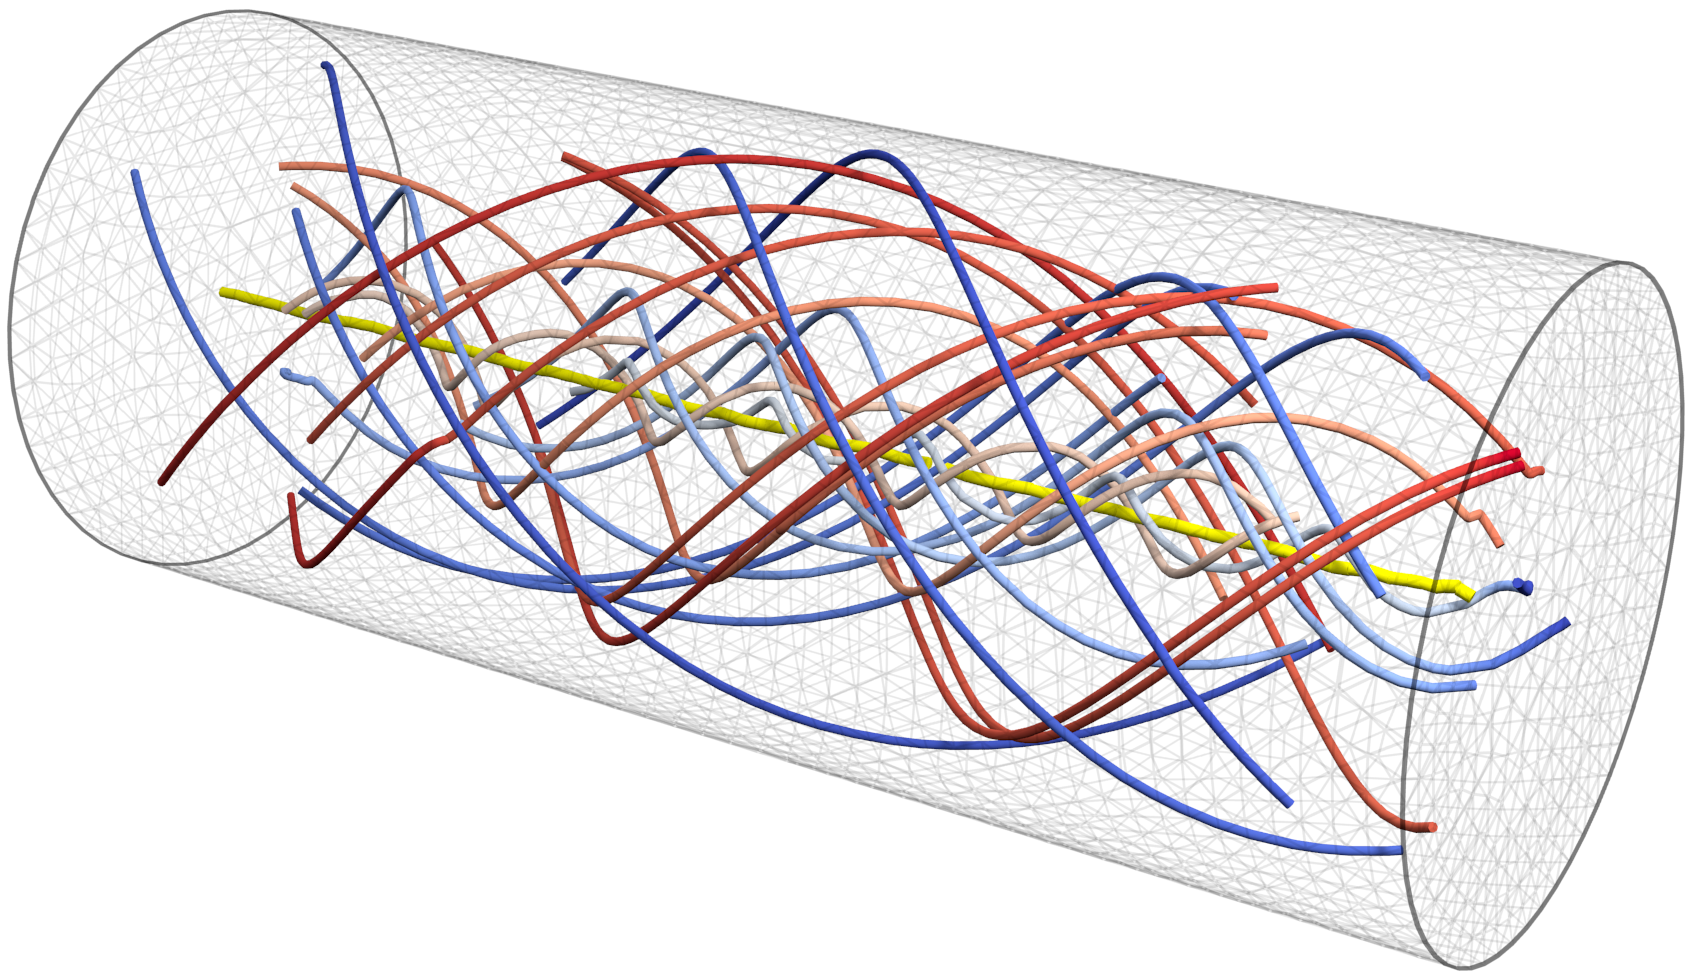
\includegraphics[width=\columnwidth]{figures/torque_tube_lines.png}
    \caption{Eigenvector trajectories in a stress tensor field induced by
             applying a torque to a cylindrical shaft. Trajectories of both
             major (blue) and minor (red) eigenvectors show a swirling behavior
             around a common core line (yellow).
             \Todo[inline]{change color scale to be consistent with other figures,
                           add arrows to indicate twist}}
    \label{fig:tube_lines}
\end{figure}
%
In particular, we make the following contributions:
%
\begin{itemize}
    \item  We give a rigorous definition of tensor core lines and show that the
    definition gives indeed structurally stable line structures.
    %
    \item We provide a numerical algorithm for the extraction of tensor core
    lines in piecewise linear tensor fields.
    %
    \item We introduce a filter criterion based on numerical stability to
    separate significant and insignificant tensor core lines.
    %
    \item We show tensor core lines in mechanical stress tensor fields,
    interpret them and compare them with degenerate lines where two eigenvalues
    are equal.
\end{itemize}
%
%
\Todo[inline]{Make connection with PEV. This algorithm simpler variant. PEV
also implementable in terms of this algorithm.}
%
\Todo[inline]{summarize sections}
%
% section introduction (end)